\section{Motivation}
\label{section_3}

%%%%%%%%%%%%%%%%%%%%%%%%%%%%%%%%%%%%%%%%%%%%%%%%%%
\begin{figure}[t]
\centering
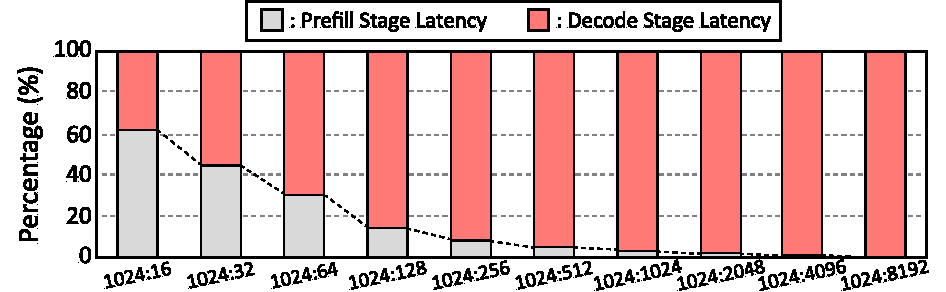
\includegraphics[width=\colimgwidth]{Figures/3_1_Prefill_Decoding_Ratio.pdf}
\caption{A latency ratio of prefill stage and decode stage in single batch Llama3-8B inference on RTX 4090. Total is 100\% and the X-axis means the number of input tokens: output tokens}
\label{fig_3_1}
\vspace{-0.5em}
\end{figure}
%%%%%%%%%%%%%%%%%%%%%%%%%%%%%%%%%%%%%%%%%%%%%%%%%%
\subsection{Decode stage Overhead in xPU}
\label{section_3_1}

Both the prefill and decode stages must be carefully considered in the design of LLM inference systems. However, once a system is optimized for the prefill stage—typically through a highly parallel architecture—the performance bottleneck shifts to the decode stage. Most commercial GPUs and NPUs fall into this category. Figure~\ref{fig_3_1} illustrates the ratio of prefill and decode stage latencies according to token lengths on an Nvidia RTX 4090~\cite{RTX4090}. As shown in the figure, even when the number of prefill tokens and decoding tokens is identical, the decode stage accounts for 98\% of the end-to-end latency.

This imbalance is further exacerbated by the recent emergence of reasoning LLMs. Such models tend to generate significantly longer output sequences compared to conventional LLMs. Table~\ref{table_2_1} presents the context lengths produced on the GPQA-Diamond~\cite{GPQA-Diamond} benchmark by two models sharing the same base architecture. As shown, reasoning LLMs generate sequences that are approximately 2.99$\times$ to 5.20$\times$ longer than their non-reasoning counterparts. As a result, the decode stage becomes substantially prolonged, further reinforcing its dominance in overall latency.

This outcome may change in cases of large-batch inference. Nevertheless, in the case of low-batch LLM inference acceleration, prioritizing performance improvement in the decode stage is more appropriate than enhancing computational capabilities.

% For instance, hardware specialized in the decode stage processing can show suboptimal performance during the prefill stage. Conversely, there is also hardware that handles the prefill stage well but exhibits relatively weak decode stage performance due to lower memory bandwidth compared to its TFLOPS.

%%%%%%%%%%%%%%%%%%%%%%%%%%%%%%%%%%%%%%%%%%%%%%%%%%
\begin{table}[t]
    \caption{Context length comparison of various LLMs}
    % \Description{Hardware specification of NVIDIA A100 GPU and Oaken equipped with either HBM or LPDDR memory.}
    \vspace{-1.0ex}
    \centering
    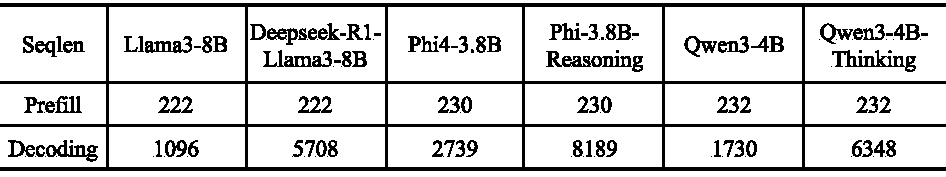
\includegraphics[width=1.0\linewidth]{Tables/2_2_Reasoning_TokenLength.pdf}
    \label{table_2_1} 
    \vspace{-1.5em}
\end{table}
%%%%%%%%%%%%%%%%%%%%%%%%%%%%%%%%%%%%%%%%%%%%%%%%%%

\subsection{Significant Accuracy Drop from Lossy Compression in Modern LLMs with Reasoning Capability}
\label{section_3_2}

% the decode stage acceleration methods we can consider are either adopting hardware with higher memory bandwidth or utilizing lossy compression. As the cost and power issues associated with high memory bandwidth hardware make them practically unsuitable for consumer-grade devices

In edge LLM inference scenarios with limited batching, lossy compression has been widely adopted as a primary acceleration technique. While effective in improving performance, lossy compression inevitably introduces accuracy degradation, and most existing approaches focus on minimizing this loss. However, techniques that are reported to incur negligible degradation on standard benchmarks often fail to generalize to more challenging tasks, where the resulting accuracy drop becomes substantial.

Table~\ref{6_2_accuracy_table} in section \ref{section_6_2} presents the measured accuracy after applying several state-of-the-art lossy compression techniques to various reasoning LLMs. As shown in the table, even lossy compressions that exhibit little performance degradation on relatively easy benchmarks suffer non-negligible performance drops on complex reasoning benchmarks.

This observation does not invalidate the overall effectiveness of lossy compression. Techniques such as quantization and pruning continue to provide significant performance gains while maintaining acceptable accuracy for less demanding workloads. However, considering that most recent small LLMs possess reasoning capabilities, and in contrast, quantization and pruning research is increasingly proposing aggressive techniques, relying solely on lossy compression going forward is not appropriate. To fully harness the performance of state-of-the-art LLMs in an edge environment, a method to accelerate low-batch LLMs while maintaining accuracy is absolutely essential.




\subsection{Potentials of Speculative Decoding and Limitations of Current Methods in Edge LLM Inference Environment}
\label{section_3_3}

Given the absence of a definitive solution for optimizing edge LLM inference, speculative decoding emerges as a promising approach for accelerating LLMs on consumer-grade xPUs. However, existing research on speculative decoding has primarily targeted large-scale models deployed in server environments, leaving several challenges unresolved in edge settings.

The most critical limitation is that many speculative decoding approaches rely on additional training. Although recent methods have reduced the training cost, such requirements remain impractical for users with resource-constrained devices. For instance, Eagle-3 speculative decoding model~\cite{eagle3}, a state-of-the-art training-based approach, requires approximately two days of training on four NVIDIA A100 GPUs to construct the draft model. This level of computational demand presents a significant barrier for edge users, who typically operate with limited hardware resources.

%%%%%%%%%%%%%%%%%%%%%%%%%%%%%%%%%%%%%%%%%%%%%%%%%%
\begin{table}[t]
    \caption{Comparison of different speculative decoding methods}
    % \Description{We can see serious accuracy drop.}
    \vspace{-1.0ex}
    \centering
    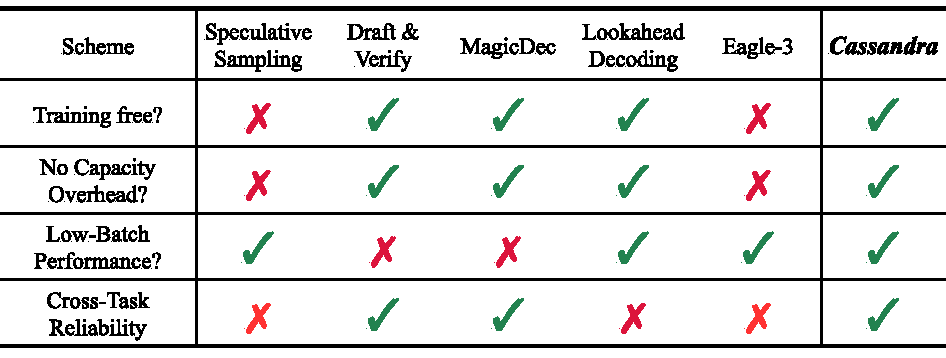
\includegraphics[width=1.0\linewidth]{Tables/3_3_Speculative_Decoding_Comparison_Table.pdf}
    \label{table_3_3_speculative decoding} 
    \vspace{-3.0ex}
\end{table}
%%%%%%%%%%%%%%%%%%%%%%%%%%%%%%%%%%%%%%%%%%%%%%%%%%

To address these issues, recent studies have explored training-free self-speculative decoding~\cite{Draft&Verify, QuantSpec, MagicDec}. These approaches construct the draft model directly from the original model, eliminating the need for additional training. For example, Draft\&Verify~\cite{Draft&Verify} generates draft outputs via layer skipping, while MagicDec~\cite{MagicDec} leverages sparse retrieval of the KV cache. Despite their advantages, existing self-speculative methods typically rely on coarse-grained approximations and primarily focus on reducing overhead in the attention mechanism and KV cache. As a result, although they demonstrate reasonable performance in batched inference scenarios, their benefits are often limited in low-batch, small-model settings that are common in edge environments.

In addition, several speculative decoding methods~\cite{speculativesampling, eagle3} employ independent draft models with separate weights and KV caches. This design introduces non-negligible memory overhead, which is particularly problematic for resource-constrained devices, as it reduces the maximum feasible sequence length under a fixed memory budget.

As summarized in Table~\ref{table_3_3_speculative decoding}, existing speculative decoding approaches exhibit distinct trade-offs, and no single method fully satisfies the requirements of edge deployment. Therefore, we propose Cassandra, a novel approach designed to overcome these limitations and enable efficient speculative decoding in edge LLM inference scenarios.

% Moreover, the effectiveness of training-based speculative decoding is highly dependent on the training data distribution, leading to inconsistent performance across tasks. As illustrated in Figure~\ref{fig_7_1} (Section~\ref{section_7_2}), Eagle-3 exhibits a notably low acceptance rate in long-context scenarios. Considering that long-context reasoning has become a key direction in modern LLM development, this limitation significantly undermines its practicality.

% To overcome these drawbacks, some studies have proposed training-free self-speculative decoding~\cite{Draft&Verify, QuantSpec, MagicDec}. Self-speculative decoding is the idea of using a part of the original model as the draft model. While some self-speculative decoding methods~\cite{Kangaroo} require fine-tuning, the majority are training-free. For instance, Draft\&Verify~\cite{Draft&Verify} implemented the draft model by employing layer skipping on the original model, and MagicDec~\cite{MagicDec} constructed the draft model by sparsely retrieving a portion of the original model's KV cache. However, the problem is that existing self-speculative methods generally employ coarse-grained draft model generation techniques and primarily focus on reducing the overhead of only the attention layer and KV cache. Consequently, despite showing decent performance in batched LLM environments, these methods usually show limited performance in low-batch, small LLM inference settings.

% Finally, some speculative decoding~\cite{speculativesampling, eagle3} methods use an independent draft model and store its weights and KV cache completely separate from the original model. This approach poses a potential memory capacity overhead on resource-constrained devices, ultimately reducing the possible length of the token sequence that can be generated by the same model.

% As shown in Table~\ref{table_3_3_speculative decoding}, different speculative decoding methods face different challenges, and there is no ultimate solution for edge-level speculative decoding. Therefore, we propose Cassandra, a novel solution that satisfies all of these requirements to enable the wider adoption of speculative decoding in the edge LLM inference environment.